%% marcel's template

\documentclass[12pt]{article}
\usepackage[margin=0.5in]{geometry}
\usepackage{amsmath,amsthm,amssymb,amsfonts,tikz,tikzsymbols}
\usepackage[shortlabels]{enumitem}

\usepackage{hyperref}

\newenvironment{rcases}
  {\left.\begin{aligned}}
  {\end{aligned}\right\rbrace}

\newcommand{\N}{\mathbb{N}}
\newcommand{\Z}{\mathbb{Z}}
\newcommand{\Q}{\mathbb{Q}}
\newcommand{\R}{\mathbb{R}}
\newcommand{\C}{\mathbb{C}}
\newcommand{\F}{\mathbb{F}}
\newcommand{\RA}{\Rightarrow}
\newcommand\defeq{\mathrel{\stackrel{\makebox[0pt]{\mbox{\normalfont\tiny def}}}{=}}}

\newcommand{\M}{\mathbb{M}}

\renewcommand\qedsymbol{$\Smiley$}

\newenvironment{problem}[2][Question]{\begin{trivlist}
\item[\hskip \labelsep {\bfseries #1}\hskip \labelsep {\bfseries #2.}]}{\end{trivlist}}
\newenvironment{exercise}[2][Exercise]{\begin{trivlist}
\item[\hskip \labelsep {\bfseries #1}\hskip \labelsep {\bfseries #2.}]}{\end{trivlist}}
%If you want to title your bold things something different just make another thing exactly like this but replace "problem" with the name of the thing you want, like theorem or lemma or whatever

\begin{document}
 
%\renewcommand{\qedsymbol}{\filledbox}
%Good resources for looking up how to do stuff:
%Binary operators: http://www.access2science.com/latex/Binary.html
%General help: http://en.wikibooks.org/wiki/LaTeX/Mathematics
%Or just google stuff
 
\title{DATA SILSO HISTO quality control Report}
\author{Stephen Fay}
\maketitle

\section{Introduction}
\subsection{Github repository and project}
    https://github.com/dcxSt/DATA\_SILSO\_HISTO\_search \\
    https://github.com/users/dcxSt/projects/2?fullscreen=true
    
\subsection{Brief History et Mise en Contexte}

For centuries we have observed the sun and it's ever mysterious sunspots. The 11 year sunspot cycle has long been a subject of debate. Today we wish to have precise quantification of solar activity throughout the previous centuries. This is made possible by the sunspot series. For the past 3 to 4 hundred years people all over the Eurasian continent have been recording the number of sunspots that appear on the sun's earth facing half. 

The aim of this project is to do a quality control of the data in DATA\_SILSO\_HISTO. Once the data is fixed and cleaned up, it will be stored on a new database - temporarily named GOOD\_DATA\_SILSO in a more user-friendly format to what currently exists. I will also get rid of any useless or redundant columns (such as the observers comment column - there are no comments )': ). A third, temporary database will be mad to keep a closer eye on the data that still needs to be examined with more scrutiny : BAD\_DATA\_SILSO. This database will act as intermediary between DATA\_SILSO\_HISTO and GOOD\_DATA\_SILSO. We will effectively be storing 2 databases-worth of information in 3 databases. The original DATA\_SILSO\_HISTO will have the old data and will be corrected in due course. The intermediary BAD\_DATA\_SILSO will start as a copy of DATA\_SILSO\_HISTO and end up empty as the corrected data is removed from it and placed, in the new format, into GOOD\_DATA\_SILSO.


\section{Processus de filtration / corigee du data (log) / quality control}

\subsection{Everything wrong with the data}

First, it's important to note that note that though I am doing a quality control I do not wish to die of boardom. I will not be verifying each of the 205003 data-points by hand in the Mittheilungen journals, in any case this if I went about it this way I would probably miss most of the errors.

\subsection{Annotation keys}

\subsubsection{What do the flags mean?}\label{flags section}
\newpage% idk how to make tables behave!
\begin{table}[h!]
    \centering
    \begin{tabular}{c|c|c|c|c|c|c|c|c|c}
        0 & 1 & 2 & 3 & 4 \\
        same as Null & suspicious & Comment in journal = ? & move to bin & suspiciously high\\
        \hline
        5 & 6 & 7 & 8 & 9\\
        very suspicious & misc see comment & probs ok, to be investigated & null groups & null sunspots
         
    \end{tabular}
    \caption{Flags key}
    \label{tab:flag}
\end{table}
\begin{enumerate}[start=0]
    \item The default for the flag is NULL, when is estimate that the datapoint is perfect and there is nothing wrong with it, I can put it to zero 0.
    \item If the data looks fishy but I'm not quite sure either what is wrong with it or how wrong it is this is flagged with a 1 - the default.
    \item If in the Mitteilungen journals there is written a ? next to one of the data points, I will mark it with a 2, this means that the observer is not quite confident in his/her result.
    \item A flag that signifies that this data point is definitely going into the bin
    \item For data that is very dodgy but it is ambiguous as to weather or not it is correct, to determine its validity closer examination is required
    \item For data that is definitely wrong, the difference between 5 and 4 is illustrated by example: if i find that a datapoint has a groups number of 30 I will mark it with a 4 and comment it, because this is suspicious, if a datapoint has a groups number over 60 or above, it will be marked with a 5 (trust me there are some in the hundreds).
\end{enumerate}
  


\subsection{Search and correct.}

\subsubsection{Outline}

For the first week and a half or so, I spent the bulk of the time acquainting myself with the Mittheilungen journals, and with the software that is used to store and access the database. I also developed the tools in python to facilitate my access to them and to perform the tasks that I need to perform for the filtration process. 



\subsubsection{Log}
I started this (today) on 2019.06.21 (yes, the solstice!)
\begin{itemize}
    \item Friday June 21
    \begin{itemize}
        \item Today no-one was in the office in the morning so I didn't have access to the Mittheilungen journals and decided to start writing this instead
        \item at 10:20 I was let into my bit with all my notes and the journals and began 'searching the manuals' part of the project documented in the Github project linked
        \item been spending time writing in all the pink corrections, including typos
        \item started writing 'searching\_the\_manuals.py'
        \item wrote and executed methods : def\_correct\_typos\_for\_pink() ; pink()
        \item searching the manuals for all comments labeled 'uncertain' so as to figure out what is this word's range of meaning (wishing I had paid attention in German class)
    \end{itemize}
    \item Monday June 24
    \begin{itemize}
        \item 9.15 picking up from where I left off, I am currently scouring the manuals for any 'uncertain' data
        \item 10.40 came across some duplicate data, and mysterious comments... there are some stars '*' that signify a change of instrument but nothing is written. The annoying thing about the duplicate data is that it is coming from 
        \item spent the morning making that duplicate finding and sorting algorithm, now I need to analyse the nature of the problem further. For each of the duplicates identify what kind it is, weather it's the same observer with the same instrument; if the duplicated data has for example the same rubrics numbers as each other ; if they record the same information (sunspot groups, sunspots, wolf number) ; if check to see if any clues are hidden in the comments of these duplicated data
        \item in searching\_the\_manuals i wrote : find\_duplicate\_observers() ; find\_obs\_id\_by\_date() ; find\_observer\_alias\_by\_id() ; find\_duplicates\_data() ; write\_greater\_duplicates\_data\_text()
        \item i'm gonna go and delete some of the data so i will log everything in order to be very careful
    \end{itemize}
    \item Tuesday June 25
    \begin{itemize}
        \item 9.45 I have decided to start making modifications to the database, this is risky business - I don't want to have the blood of Galileo's data on my hands, in a few seconds I can destroy hours upon hours of one of my predecessors' work. Which would be a shame. This is why I am creating a new table in both the old and the new database that will serve as a rubbish bin, so that I simultaneously copy and delete some data. The data will be copied and destroyed in the same script but the coping will come \textit{before} so if there are bugs nothing will be lost. First I will back up the databases as they are.
        \item While making the rubbish bids for DATA\_SILSO\_HISTO if found that DATA\_DEV was non-empty, it contains data which claims to be observations made by the grandfather of this series - Rudolf Wolf. Only the observations are dated January 1600 - Galileo's time, 216 years before Wolf's birth! And so I renamed the DATA\_DEV to RUBBISH\_DATA and added the flag column, leaving those four observations inside where they probably belong...
        \item Wrote a new script to deal uniquely with deleting the duplicates
        \begin{itemize}
            \item finished writing move\_data\_to\_bin and delete\_entered\_twice\_duplicates
            \item executing delete\_entered\_twice\_duplicates()... done
            \item finished commenting these data points in rubbish data in both databases
        \end{itemize}
    \end{itemize}
    \item Wednesday June 26
    \begin{itemize}
        \item wrote a new method in db\_edit for appending comments rather than replacing them
        \item wrote \textit{unreasonable\_sn\_flag()} a method that takes a look at the groups number and the sunspots number of each entry and determines if it's realistic or not. I decided somewhat arbitrarily that if the groups number was higher than 30 it would be flagged with flag 4, if the groups number was higher than 60 it would be marked with a 5 this is beyond unreasonable. I did something similar for the sunspots number $sunspots>100\Rightarrow flag:=4$ and $sunspots>250\Rightarrow flag:=5$ (see the flags section \ref{flags section}). The method was executed and ran without a hitch (after a bit of debugging)
        \item just set another 212 flags for putting things in the bin. There are still 4000 pairs of duplicates that need attending to but considering i started with 14000 that's not bad... Some of the duplicates may be left as they are. Also i figured out that i had flagged some which just had a 0 sunspot number and so i went and unflagged them.
        \item i spent alot of time scrutinising what i had flagged, rereading my scripts, seeing that I've been using really inefficient algorithms, checking things are in the right place. And wondering how on earth many things ended up with the flags they ended up with.
        \item something that has been annoying me in this search is I can't seem to be able to determine what is an unreasonable number of sunspots that can appear on the sun, because many many observer record having over 250. This is why I will start using graphical tools to help me figure all of this out. I will make the graphs in a jupyter notebook.
    \end{itemize}
    \item Thursday June 27
    \begin{itemize}
        \item first thing i did today is to go though and look at lots of the flagged data from yesterday on the mysql databases
        \item Panic! While searching I came across a big problem. Many of the datapoints are labelled '*' in the comments, this corresponds to when there is an asterix in the Mitteilungen journals, but here's the twist: the star is usually a reference to the fact that there is a change in the observer's telescope to his/her secondary lunette. This is written nowhere is many cases in the digital database! This is a new task I must take on am I to accomplish my mission here:
        \begin{enumerate}
            \item Correct all the comments so that they display useful information i.e. '*' --- '* = 8 cm Oeffnung mit 64-facher Vergrosserung und Polarisationshelioscop'
            \item When you tackle the 'Creating New Aliases' part of the project (see my Github - username = dcxSt - project sun)
        \end{enumerate}
        \item I found there I had flagged all the mysterious '*' comment 1 and that none of them have found their way into my pristine database GOOD\_DATA\_SILSO and so I went through each of them individually and wrote the changes that I implemented in the python method 'correct\_asterix\_comments()' in script 'db\_homogenise\_comments.py'. This took quite some time and included translating German with my good friend google-translate. This corrected about 250 data-points' comments (i didn't bother to count)
        \item after a long search of the data in GOOD\_DATA\_SILSO with FLAG=3 which have no superior duplicates I found that these were infact correctly flag and that their double had not yet made it into my new database because there were commented (usually with an asterisk *) so i moved them into the bin
        \item Found a bug in move\_flag3\_to\_bin() which may have been causing some of the perplexing problems I had earlier
        \item I ran the method 'flag\_many\_duplicates()' many times using the duplicates text files I'd made earlier for inspiration to change it subtly so as to catch those sneaky no good duplicates!
        \item IMPORTANT: I just found some data which has been written in in the wrong year. In rubrics 820 students have mistakenly typed in the data for Wolfer in the year 1900 and written it in the year 1899.
        \item In the folder duplicates/3 2019.06.27 I am writing the file corrections\_needed\_handwritten.txt which outlines the corrections which are to be made to the data if we want to solve some of these duplicates.
    \end{itemize}
    \item Friday June 28 
    \begin{itemize}
        \item Continued what I was writing yesterday, looking through the manuals and identifying. The notes I took about the duplicates can be found in different\_value\_duplicates.txt, some things I found interesting so I decided to copy most of the file into this report
        \item Carrington datapoint id=31460 needs to go in the bin this is clearly a penumbra
        \item All observations in rubric number = 808 with fk\_rubrics = 461 were made by Konkoly not Wolfer
        \item All observations in rubric number = 820 were made by Wolfer in the year 1900 and not 1899, many observations are written correctly except for the year of the date, I found that the months and days correspond perfectly with what is written in the journals but not the year!
        \item The Broger duplicates for 1899-03-17 and 1899-04-18 make very little sense, they are broger under two different aliases but in the same rubrics 801. There are only two of them so they can be done by hand. My guess is that they were punched in twice by different people and my identical duplicates algorythem has already dealt with the ones that were exactly the same, so these are the 2 instances where one of the people got it wrong.
        \item Observations in mitt 129 rubrics number 02 (or 12902) were all made by Broger in 1931. Manny if not all of them were typed in wrong, it says they were made in 1908. Thankfully everything else about them seems correct.
        \item For Rubrics 1057 and 1058 there is a serious problem - Both are labled with the wrong observer! 
        \begin{itemize}
            \item Rubrics number 1057, the observations are made in the Capodimonte Observatory by Dr. E. Guerrieri,
            \item Rubrics number 1058, the observations are made in Floreze by Robert Lucchini. I checked and both of these boyz are real observers with aliases, so this needs to be corrected.
            \item The reason there is confusion about these two is because Herrn J. Sormano in Turin is mentioned since the observations come from letters of correspondence between Sormano and the two observers mentioned above. It is quite possible that this has been going on in other places under the radar. The only reason these two were detected was because they just so happened to be attributed to the same guy for observations on the same date. What I propose is that we have someone (perhaps me, Asside: maybe an AI could do this if we scanned every page of the journals and then trained a neural net to read the rubrics descriptors and figure the observer based on that... This might be hard for this task but I can see how some machine learning could come in handy for error detection and quality control) go through each rubrics number and make a list where every rubrics number is ascribed to an observer, specially for the rubrics descriptors that include the names of several people, come to think of it a German person would proably do a much better job at this then me.
            \item To speculate further it is possible that this issue runs deep and that many of the holes in the data are infact a concequence of the kind of error described above (by the way I can cut out alot of my rambling from the final draght of the report, or make a condensed version, I'm just in the habit of writing everything down so that future me can follow the thought process, sometimes it helps ok!)
    \end{itemize}
    \item Observations from rubrics number 1279 were incorrectly labled as comming from 1919 when infact they are from 1920. The observer (Prof. Anne Young) and all other info is correct.
    \item Something annoying happens in 1929, Both Brunner - 'Wm. Brunner'  and his assistant - 'W. Brunner, Assistent' seem to be observing at the same time [BOTH OF THEM ARE DENOTED WITH THE ALIAS 'Brunner'] with the same 8 cm aperture 64x magnification polarised helio-telescope. Rubrics 1624 (fk\_rubrics=840) is Brunner and his assistent's observations are from Rubrics 1675 (fk\_rubrics=842). I don't know what we should do, perhaps create another alias 'Brunner Assistent' (pink page marker)
    \begin{itemize}
        \item Same thing happens in rubrics 12501 (fk=844) is the real Brunner, and rubrics 12503 (fk=846), this is Brunner Assistent (yellow page marker).
        \item Same again in 1931. Rubrics 12901 (fk=848) is the real Brunner, and rubrics 12903 (fk=962), this is Brunner Assistent (orange page marker)
        \item ...This goes on until (see the file for details)...
        \item And in 1944. Rubrics 14401 (fk=1006) is the real Brunner, and rubrics 14402 (fk=1007) is Brunner Assistent. (green page-marker on page 112)
        \item Comments on Brunner: I'm annoyed that the assistant(s) doesn't have a name because we now have no idea how many there where. Also (s)he deserves credit for those 10 odd years of commited observation! Because this assistent has been observing with Brunner from 1929 to 1944 he at least deserves an alias. 
    \end{itemize}
    \item Messerschmitt and Wasnetzoff
    \begin{itemize}
        \item Something strange happens with Messerschmitt, there are two different sunspots values written in for 1908-02-15, one of them has no rubrics number and values 3,17,47 The other has a rubrics number 1028 and values 2,7,27. So I looked in the journals under rubrics 1027 and for this date I found the values 3,17,47 which are the values written in where no rubric is specified. Very strange. There are a total of 4 duplicates for Messerschmitt and this is the only one that has a rubrics number. I find this very strange... I don't really know what to do. 
    \end{itemize}
    \end{itemize}
    
    \item Monday July 1
    \begin{itemize}
        \item Using what I did on Friday (wrote that list of things that were wrong with specific duplicates) to bin some data and modify other data
        \item Started writing methods flag3\_from\_correction\_txt() and change\_rubric\_observer() and change\_date\_rubric() in dealing\_with\_duplicates.py, and then I realised that all this was much simpler and could be done faster and less error prone if I just punched in the queries to through mysql directly, so this is what I did.
        \item With care and delicacy I changed the observer aliases / and for the old and bad database I changed the FK\_OBSERVERS with the terminal. Now I move onto changing all the faulty dates, this requires a bit of coding because I need to loop through the dates and change each date individually.
        \item Wrote change\_dates() and it's helper change\_date\_rubric() (in dealing\_with\_duplicates.py) and executed them in more time than it should have taken. My head is not clear today, but I was rigourouse, there should not be a mistake.
        \item I am changing the databases quite a bit so I saved a new backup file
        \item made a new alias in DATA\_SILSO\_HISTO (and BAD\_DATA\_SILSO) called `Brunner Assistent'. I know the name lacks imagination but hey (I couldn't find who it might be online - future me : this is a reminder to ask Frederic if he might know, be ready with dates...).
        \item I just realised that when I was changing some of the data in GOOD\_DATA\_SILSO I only changed the aliases, to correct this I will either write now or once everything is finished a method that goes through each data-point finds the alias and corrects the observer data (things such as the country of observation, the observer comments and the instrument etc.)
        \item wrote and executed the command in dealing\_with\_duplicates.py change\_alias\_to\_brunner\_assistent(), this corrected the brunner assistent problem we had
        \item backed up the the databases to sql files
        \item I realised that I had missed correcting the alias for rubrics 195 from Franzenau to Weber so I did that just now
        \item Ran the method that shows me what is wrong with the duplicates to see how effective my cleanup has been : interesting, the duplicates that were Weber's but marked Franzenau had already been entered under Weber but with rubrics\_number=0 and no references in the Mittheilungen, so I reran the flag\_many\_duplicates.
        \item Some of the 'Tacchini and Milesovich' are missing sources but the duplicates are identical, so I moved one from each to the rubbish bit by calling the method delete\_entered\_twice\_duplicates() from dealing\_with\_duplicates.py. There was also the issue that Broger had some identical data typed in for him in two using two different observer ids that both refer to him... so i added an elif statement into the delete entered twice duplicates method to deal specifically with this.
        \item Most of this data has been cleaned up, the rest can be done by hand
    \end{itemize}
    
    \item Tuesday July 2
    \begin{itemize}
        \item exploring ways of creating visualisations that will help me catch some of the suspicious data-points. Right not my task is hunting down those ones which I labelled 'suspicious sunspots'
        \item made some pretty plots which you can find in \textit{suspicious sunspots plots.ipynb} in the root directory
        \item Using the plot I was able to check some of Weber's suspicious sunspots in the Mittheilungen. And strangely enough Weber's observations are correct! It seems he really did see 476 sunspots on the sun on the 25th of september 1870. I mean the patter fits it's just unsusually large. And you need to be dedicated to count hundreds of spots every day.
        \item Made a method in the jupyter notebook mentioned above that plots an observer's stuff and color codes the flags. I investigated Tacchini's green (flag=4) datapoints and they are infact correct, they appear in the journals. There is one datapoint from Tacchini which I corrected by hand, this one had a wolf number of 61, I found it in the journals, the correct value was 6 - typo. I corrected it manually.
        \item In the rubric 279 mitt 30 page 409 Tacchini observes a bunch of sunspots without observing any groups. This is annoying because it means we have no wolf! Other than that they seem to have been entered in correctly, I have not yet transfered these to the GOOD DATA SILSO database, they are still only in DATA SILSO HISTO and BAD DATA SILSO
        \item I have an idea that we could do some stats and deduce a wolf number even without the groups, and give it a special flag, based on some probability we estimate a wolf number. There might be some complications with this tactic, here are 3 possible ways of doing it and their weaknesses:
        \begin{enumerate}
            \item For each sunspots number possible \{1,2,3...\} find the corresponding most likely wolf number by going though each data point with that number and doing a distribution (probs normal) to find which is the most likely wolf number associated with this sunspots number. Essentially we define a function term-by term $f \defeq{} \N \to \R$. The weakness : if we sample everything we might find that Tacchini has his own idiosyncratic way of doing sunspots and wolf, and so the data we add to his entriee would not fit well with his methods of observation.
            \item For each sunspots number do the same as above but go through the groups number! Again for each sunspots number find sift through all the data of everyone to find the best groups number $g\in \R$, i.e. the $g$ s.t. it sits on top of the fitted normal distribution.
            \item For each sunspots number, methods 1) and 2) above but fitted with only Tacchini's previous and future data. The weakness of this method is that there is not much data to go on... (relative to the first two)
            \item One thing that worries me in the case of Tacchini is that this guy observers a lot of sunspots. I am looking at his entries right now and in 1870 he regularly observers over 200 sunspots, on $5^{th}$ of April 1870 he sees 302 sunspots. That said cross-referencing his data with other observers' from the same time seems to support this hypothesis. But the more sunspots he observers, the less data we have to make a nice normal distribution for each sunspots number, there may be sunspots numbers that only appear like 3 times in the whole database, how are we to do any stats on those. The answer is the following method for tying sunspots to groups and wolf number: for each sunspots number we link it to a wolf number by finding the best fit normal distribution for the likeliest wolf number to be associated with it. Then we give this value an error bar which is bigger the less data we have. Then we do a plot x-axis = sunspots number, y-axis = wolf numbers with vertical error bars. Then we do a line of best fit through the whole lot, try several models and do a chi-squared test. It might be worth getting rid of the small ones and only look at data where $s>20$. Again we could do this for wolf directly and for groups then wolf.
        \end{enumerate}
    \item Before embarking on this adventure I will first endeavour to plug both of Tacchini's hole's that appear in the plots I made: 3 entire years are missing From Tacchini's data 1877, 1878 and 1881
    \item In 1881 the rubrics number 465 contains two data sets, one of them is entirely Ricco's and the second is from Tacchini and G. Millosevich. Nowhere int the data set is it indicated who saw what, so I looked and found that there was no Alias for Millosevich. This makes me think that he must be Tacchini's assistant or observing partner. Anyway we have a big gap in Tacchini's observations, what I will do is comment all of these observations ``Tacchini and Millosevich". I did that and gave them a flag, then regenerated the Tacchini graphs and there is no more gap in 1881, what's more the data looks almost identical. There is one only slightly worrying difference and maybe I'm inventing patterns where I am trying to see them but the 1881 observations are on average a tiny tiny bit higher than the surroundings. Actually I will put a picture \textbf{here (put link to picture I will include in this report)}, I think this is infact a seasonal effect, there is more atmosphere...
    \end{itemize}
    \item I improved the jupyter notebook ``suspiciou sunspots plots.ipynb", made a cool colour scheme for the various flags, and you should definitely \textbf{check this out (link of tacchini pink patches with flag=6)}
    
\end{itemize}

\subsubsection{Python scripts - what they contain}



\section{Comparaison du data avant et apres + visualisations}

\subsubsection{The original sql data tables format}

\begin{table}[h!]
    \centering
    \caption{DESCRIBE DATA}
    \begin{tabular}{c|c|c|c|c|c}% l c r = Left Centre Right
        \textbf{Field} & \textbf{Type} & \textbf{Null} & \textbf{Key} & \textbf{Default} & \textbf{Extra}  \\
        \hline
        ID & int(11) & No & PRI & NULL & auto\_increment \\
        
        DATE & date & YES && NULL & \\
        
        FK\_RUBRICS & int(11) & YES & MUL & NULL &  \\
        
        FK\_OBSERVERS & int(11) & YES & MUL & NULL &  \\
        
        GROUPS & int(11) & YES && NULL &  \\
        
        SUNSPOTS & int(11) & YES && NULL & \\
        
        WOLF & int(11) & YES && NULL &  \\
        
        QUALITY & int(11) & YES && NULL &  \\
        
        COMMENT & text & YES && NULL &  \\
        
        DATE\_INSERT & datetime & YES && NULL &  \\
        
        FLAG (i added this) & tinyint(1) & YES && NULL &  \\
        
    \end{tabular}
    \label{tab:data-og}
\end{table}

\begin{table}[h!]
    \centering
    \caption{DESCRIBE OBSERVERS}
    \begin{tabular}{c|c|c|c|c|c}% l c r = Left Centre Right
        \textbf{Field} & \textbf{Type} & \textbf{Null} & \textbf{Key} & \textbf{Default} & \textbf{Extra}  \\
        \hline
        ID & int(11) & NO & PRI & NULL & auto\_increment \\
        
        ALIAS & varchar(50) & YES && NULL & \\
        
        FIRST\_NAME & varchar(50) & YES && NULL &  \\
        
        LAST\_NAME & varchar(50) & YES && NULL &  \\
        
        COUNTRY & varchar(50) & YES && NULL &  \\
        
        INSTRUMENT & varchar(50) & YES && NULL & \\
        
        COMMENT & text & YES && NULL &  \\
        
        DATE\_INSERT & datetime & YES && NULL &  \\
        
    \end{tabular}
    \label{tab:data-og}
\end{table}

\begin{table}[h!]
    \centering
    \caption{DESCRIBE RUBRICS}
    \begin{tabular}{c|c|c|c|c|c}% l c r = Left Centre Right
        \textbf{Field} & \textbf{Type} & \textbf{Null} & \textbf{Key} & \textbf{Default} & \textbf{Extra}  \\
        \hline
        RUBRICS\_ID & int(11) & NO & PRI & NULL & auto\_increment \\
        
        RUBRICS\_NUMBER & int(11) unsigned & NO && NULL & \\
        
        MITT\_NUMBER & int(11) unsigned & NO && 0 &  \\
        
        PAGE\_NUMBER & int(11) unsigned & YES && NULL &  \\
        
        SOURCE & text & NO && NULL &  \\
        
        SOURCE\_DATE & date & YES && NULL & \\
        
        COMMENTS & text & YES && NULL &  \\
        
        DATE\_INSERT & datetime & YES && NULL &  \\
        
        NB\_OBS & int(11) & YES && NULL & \\
        
    \end{tabular}
    \label{tab:data-og}
\end{table}

\newpage{}

\subsubsection{My new sql data table format}

\begin{table}[h!]
    \centering
    \caption{DESCRIBE DATA (the only table)}
    \begin{tabular}{c|c|c|c|c|c}% l c r = Left Centre Right
        \textbf{Field} & \textbf{Type} & \textbf{Null} & \textbf{Key} & \textbf{Default} & \textbf{Extra}  \\
        \hline
        ID & int(11) unsigned & No & PRI & NULL & auto\_increment \\
        
        DATE & date & YES && NULL & \\
        
        GROUPS & int(11) & YES && NULL &  \\
        
        SUNSPOTS & int(11) & YES && NULL & \\
        
        WOLF & int(11) & YES && NULL &  \\
        
        COMMENT & text & YES && NULL &  \\
        
        DATE\_INSERT & datetime & YES && NULL &  \\
        
        OBS\_ALIAS & varchar(50) & YES && NULL & \\
        
        FIRST\_NAME & varchar(50) & YES && NULL & \\
        
        LAST\_NAME & varchar(50) & YES && NULL & \\
        
        COUNTRY & varchar(50) & YES && NULL & \\
        
        INSTRUMENT\_NAME & varchar(50) & YES && NULL & \\
        
        RUBRICS\_NUMBER & int(11) & YES && NULL & \\
        
        MITT\_NUMBER & int(11) & YES && NULL & \\
        
        PAGE\_NUMBER & int(11) & YES && NULL & \\
        
        FLAG & tinyint(1) unsigned & YES && NULL &  \\
        
        RUBRICS\_SOURCE & text & YES && NULL & \\
        
        RUBRICS\_SOURCE\_DATE & date & YES && NULL & \\
        
    \end{tabular}
    \label{tab:data-og}
\end{table}





\newpage{}

\subsubsection{Graphs and visual representations}

As you can see, there are some famous legends in solar science such as Carrington and Kew who were able to see over 4000 sunspots at once on a single face of the sun with their crappy telescopes that they had in the 19th century!
\begin{figure}
  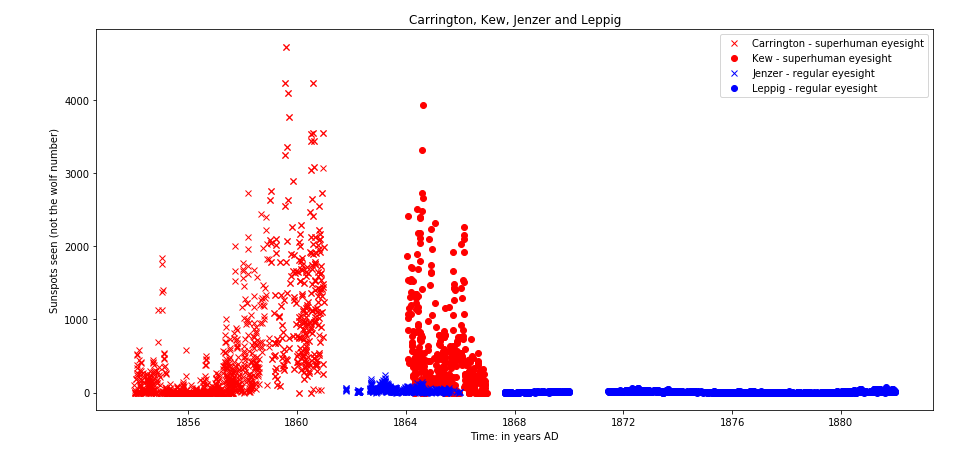
\includegraphics[width=\linewidth]{CarringtonHasGoodEyesight.png}
  \caption{Carrington has great eyesight!}
  \label{fig:boat1}
\end{figure}

\subsubsection{Thought repository - ideas that may or may not come into fluition depending on how efficiently I work and get things that need to be done done}
\begin{itemize}
    \item make some data visualisations to compare each observer's primary and secondary observing equipment
    \item for each day / month / year find the highest observation and the lowest observations and add it to the graph so that we have like an upper bound and a lower bound. 
    \item figure out how to smooth graphs with matplotlib and make something nice out off the big mess i currently have
    \item pie chart of observers with their number of observations
    \item in the final sunspots number graph cut it into 3 or 4 sections that mark changes in the theory behind sunspots: before wolf ; time where plato's ideas of the sun being a perfect sphere still were around ; 1908 George Ellery Hale discovers the magnetic link (p14 of nature's 3rd cycle) ; 1955 eugene parker's theory (p19 of nature's 3rd cycle) ; Nasa send their probe to near the sun
\end{itemize}

\end{document}